

ID: d1b66ae6\\
$-x+y=-3.5$\\
$x+3 y=9.5$

If $(x, y)$ satisfies the system of equations\\
above, what is the value of $y$ ?

$$
\begin{array}{|c|}
\hline \frac{1}{2} y=4 \\
\hline x-\frac{1}{2} y=2 \\
\hline
\end{array}
$$

The system of equations above has solution ( $x$, $y)$. What is the value of $x$ ?\\
A. 3\\
B. $\frac{7}{2}$\\
C. 4\\
D. 6

$$
\begin{gathered}
\frac{3}{2} y-\frac{1}{4} x=\frac{2}{3}-\frac{3}{2} y \\
\frac{1}{2} x+\frac{3}{2}=p y+\frac{9}{2}
\end{gathered}
$$

In the given system of equations, $p$ is a constant. If the system has no solution, what is the value of $p$ ?

\section*{ID: b86123af}
Hiro and Sofia purchased shirts and pants from a store. The price of each shirt purchased was the same and the price of each pair of pants purchased was the same. Hiro purchased 4 shirts and 2 pairs of pants for $\$ 86$, and Sofia purchased 3 shirts and 5 pairs of pants for $\$ 166$. Which of the following systems of linear equations represents the situation, if $x$ represents the price, in dollars, of each shirt and $y$ represents the price, in dollars, of each pair of pants?\\
A.

$$
4 x+2 y=86
$$

$3 x+5 y=166$

$$
4 x+3 y=86
$$

B.

$$
2 x+5 y=166
$$

C.\\
$4 x+2 y=166$

$$
3 x+5 y=86
$$

$4 x+3 y=166$\\
D.

$$
2 x+5 y=86
$$

\section*{ID: 608eeb6e}
$$
\begin{gathered}
5 x=15 \\
-4 x+y=-2
\end{gathered}
$$

The solution to the given system of equations is $(x, y)$. What is the value of $x+y$ ?\\
A. -17\\
B. -13\\
C. 13\\
D. 17\\
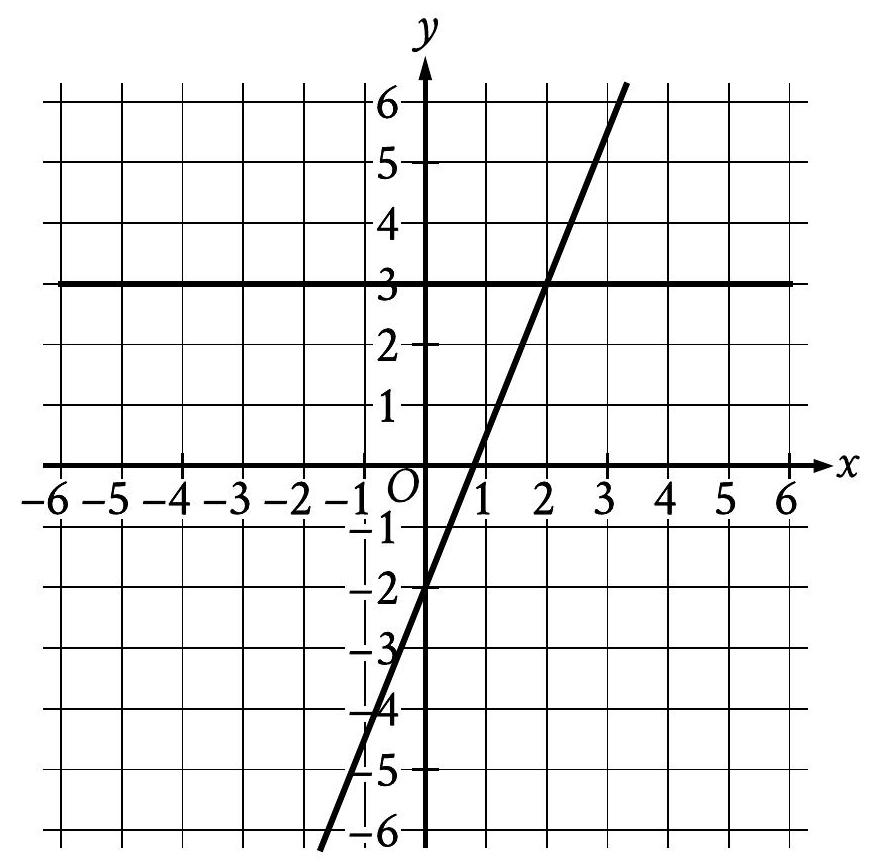
\includegraphics[max width=\textwidth, center]{2025_06_15_7d5ca6a095740ea44a32g-06}

The graph of a system of linear equations is shown. What is the solution $(x, y)$ to the system?\\
A. $(0,3)$\\
B. $(1,3)$\\
C. $(2,3)$\\
D. $(3,3)$

\section*{ID: bf4a8b6a}
A company that provides whale-watching tours takes groups of 21 people at a time. The company's revenue is 80 dollars per adult and 60 dollars per child. If the company's revenue for one group consisting of adults and children was 1,440 dollars, how many people in the group were children?\\
A. 3\\
B. 9\\
C. 12\\
D. 18

At how many points do the graphs of the equations $y=x+20$ and $y=8 x$ intersect in the $x y$-plane?\\
A. 0\\
B. 1\\
C. 2\\
D. 8

\section*{ID: 7efe5495}
$$
\begin{gathered}
y=3 x \\
2 x+y=12
\end{gathered}
$$

The solution to the given system of equations is $(x, y)$. What is the value of $5 x$ ?\\
A. 24\\
B. 15\\
C. 12\\
D. 5

\section*{ID: 71189542}
A group of 202 people went on an overnight camping trip, taking 60 tents with them. Some of the tents held 2 people each, and the rest held 4 people each. Assuming all the tents were filled to capacity and every person got to sleep in a tent, exactly how many of the tents were 2 -person tents?\\
A. 30\\
B. 20\\
C. 19\\
D. 18




































\section*{ID: 70feb725}
During a month, Morgan ran $r$ miles at 5 miles per hour and biked $b$ miles at 10 miles per hour. She ran and biked a total of 200 miles that month, and she biked for twice as many hours as she ran. What is the total number of miles that Morgan biked during the month?\\
A. 80\\
B. 100\\
C. 120\\
D. 160

\section*{ID: 8a87c2c8}
$$
\begin{gathered}
x+3=-2 y+5 \\
x-3=2 y+7
\end{gathered}
$$

The solution to the given system of equations is $(x, y)$. What is the value of $2 x$ ?\\
A. -2\\
B. 6\\
C. 12\\
D. 24

\section*{ID: ed92fb68}
$$
\begin{aligned}
& 4 x+5 y=100 \\
& 5 x+4 y=62
\end{aligned}
$$

If the system of equations above has solution $(x, y)$, what is the value of $x+y$ ?\\
A. 0\\
B. 9\\
C. 18\\
D. 38

\section*{ID: 19fdf387}
In the $x y$-plane, the graph of $y=x+3$ intersects the graph of $y=2 x-6$ at the point $(a, b)$. What is the value of $a$ ?\\
A. 3\\
B. 6\\
C. 9\\
D. 12

\section*{ID: e1248a5c}
In the system of equations below, $a$ and $c$ are constants.\\
$\frac{1}{2} x+\frac{1}{3} y=\frac{1}{6}$\\
$a x+y=c$\\
If the system of equations has an infinite number of solutions $(x, y)$, what is the value of $a$ ?\\
A. $-\frac{1}{2}$\\
B. 0\\
c. $\frac{1}{2}$\\
D. $\frac{3}{2}$

$$
\begin{aligned}
y & =4 x+1 \\
4 y & =15 x-8
\end{aligned}
$$

The solution to the given system of equations is $(x, y)$. What is the value of $x-y$ ?

ID: 52cb8ea4

$$
\begin{aligned}
& 7 x-5 y=4 \\
& 4 x-8 y=9
\end{aligned}
$$

If $(x, y)$ is the solution to the system of equations above, what is the value of $3 x+3 y$ ?\\
A. -13\\
B. -5\\
C. 5\\
D. 13

$$
\begin{gathered}
4 x=20 \\
-3 x+y=-7
\end{gathered}
$$

The solution to the given system of equations is $(x, y)$. What is the value of $x+y$ ?\\
A. -27\\
B. -13\\
C. 13\\
D. 27

\section*{ID: c5082ce3}
The score on a trivia game is obtained by subtracting the number of incorrect answers from twice the number of correct answers. If a player answered\\
40 questions and obtained a score of 50 , how many questions did the player answer correctly?

$$
\begin{gathered}
48 x-72 y=30 y+24 \\
r y=\frac{1}{6}-16 x
\end{gathered}
$$

In the given system of equations, $r$ is a constant. If the system has no solution, what is the value of $r$ ?

$$
y=4 x-9
$$

$$
y=19
$$

What is the solution $(x, y)$ to the given system of equations?\\
A. $(4,19)$\\
B. $(7,19)$\\
C. $(19,4)$\\
D. $(19,7)$

$$
\begin{gathered}
24 x+y=48 \\
6 x+y=72
\end{gathered}
$$

The solution to the given system of equations is $(x, y)$. What is the value of $y$ ?

\section*{ID: d7bf55e1}
A movie theater sells two types of tickets, adult tickets for $\$ 12$ and child tickets for $\$ 8$. If the theater sold 30 tickets for a total of $\$ 300$, how much, in dollars, was spent on adult tickets? (Disregard the \$ sign when gridding your answer.)

$$
\begin{aligned}
& x+2 y=6 \\
& x-2 y=4
\end{aligned}
$$

The solution to the given system of equations is $(x, y)$. What is the value of $x$ ?\\
A. 2.5\\
B. 5\\
C. 6\\
D. 10

$$
-15 x+25 y=65
$$

One of the two equations in a system of linear equations is given. The system has infinitely many solutions. Which of the following could be the second equation in the system?\\
A. $12 x+20 y=52$\\
B. $12 x+20 y=-52$\\
C. $-12 x+20 y=52$\\
D. $-12 x+20 y=-52$

$$
\begin{gathered}
x=5 \\
y=x-8
\end{gathered}
$$

Which of the following points $(x, y)$ is the solution to the given system of equations in the $x y$-plane?\\
A. $(0,0)$\\
B. $(5,-3)$\\
C. $(5,-8)$\\
D. $(5,8)$

\section*{ID: ffb371f5}
$$
\begin{gathered}
3 x=12 \\
-3 x+y=-6
\end{gathered}
$$

The solution to the given system of equations is $(x, y)$. What is the value of $y$ ?\\
A. -3\\
B. 6\\
C. 18\\
D. 30

\section*{ID: ece00725}
Connor has $c$ dollars and Maria has $m$ dollars. Connor has 4 times as many dollars as Maria, and together they have a total of $\$ 25.00$. Which system of equations represents this situation?\\
A. $c=4 m$\\
$c+m=25$\\
B. $m=4 c$\\
$c+m=25$\\
C. $c=25 m$\\
$c+m=4$\\
D. $m=25 c$\\
$c+m=4$

A wire with a length of 106 inches is cut into two parts. One part has a length of $x$ inches, and the other part has a length of $y$ inches. The value of $x$ is 6 more than 4 times the value of $y$. What is the value of $x$ ?\\
A. 25\\
B. 28\\
C. 56\\
D. 86

$$
\begin{aligned}
& 5 x+14 y=45 \\
& 10 x+7 y=27
\end{aligned}
$$

The solution to the given system of equations is $(x, y)$. What is the value of $x y$ ?

$$
\begin{aligned}
& 6 x+7 y=28 \\
& 2 x+2 y=10
\end{aligned}
$$

The solution to the given system of equations is $(x, y)$. What is the value of $y$ ?\\
A. -2\\
B. 7\\
C. 14\\
D. 18

\section*{ID: ee031767}
A dance teacher ordered outfits for students for a dance recital. Outfits for boys cost $\$ 26$, and outfits for girls cost $\$ 35$. The dance teacher ordered a total of 28 outfits and spent $\$ 881$. If $b$ represents the number of outfits the dance teacher ordered for boys and $g$ represents the number of outfits the dance teacher ordered for girls, which of the following systems of equations can be solved to find $b$ and $g$ ?\\
$26 b+35 g=28$\\
A. $b+g=881$\\
$26 b+35 g=881$\\
B. $b+g=28$\\
C. $\begin{aligned} & 26 g+35 b=28 \\ & b+g=881\end{aligned}$\\
D. $\begin{aligned} & 26 g+35 b=881 \\ & b+g=28\end{aligned}$

ID: 466b87e3

$$
\begin{aligned}
& y=\frac{1}{2} x+8 \\
& y=c x+10
\end{aligned}
$$

In the system of equations above, $c$ is a constant. If the system has no solution, what is the value of $c$ ?

\section*{ID: cd33b015}
$x+y=20$\\
$2(x+y)+3 y=85$\\
If $(x, y)$ is the solution to the given system of equations, what is the value of $y$ ?\\
A. 10\\
B. 15\\
C. 60\\
D. 65

ID: e2e3942f\\
$y=2 x+1$\\
$y=a x-8$

In the system of equations above, $a$ is a constant. If the system of equations has no solution, what is the value of $a$ ?\\
A. $-\frac{1}{2}$\\
B. 0\\
C. 1\\
D. 2

$$
\begin{gathered}
8 x+7 y=9 \\
24 x+21 y=27
\end{gathered}
$$

For each real number $r$, which of the following points lies on the graph of each equation in the $x y$-plane for the given system?\\
A. $\left(r,-\frac{8 r}{7}+\frac{9}{7}\right)$\\
B. $\left(-\frac{8 r}{7}+\frac{9}{7}, r\right)$\\
C. $\left(-\frac{8 r}{7}+9, \frac{8 r}{7}+27\right)$\\
D. $\left(\frac{r}{3}+9,-\frac{r}{3}+27\right)$

\section*{ID: 4ec95eab}
$$
\begin{gathered}
y=-3 x \\
4 x+y=15
\end{gathered}
$$

The solution to the given system of equations is $(x, y)$. What is the value of $x$ ?\\
A. 1\\
B. 5\\
C. 15\\
D. 45

\section*{ID: 1e11190a}
Store A sells raspberries for $\$ 5.50$ per pint and blackberries for $\$ 3.00$ per pint. Store B sells raspberries for $\$ 6.50$ per pint and blackberries for $\$ 8.00$ per pint. A certain purchase of raspberries and blackberries would cost $\$ 37.00$ at Store A or $\$ 66.00$ at Store B. How many pints of blackberries are in this purchase?\\
A. 4\\
B. 5\\
C. 8\\
D. 12

\section*{ID: e77a76ce}
Which of the following systems of linear equations has no solution?

$$
\text { A. } \begin{aligned}
y & =6 x+3 \\
y & =6 x+9
\end{aligned}
$$

B. $y=10$

$$
y=10 x+10
$$

C. $y=14 x+14$

$$
y=10 x+14
$$

D. $x=3$

$$
y=10
$$

\section*{ID: b3c7ca1d}
Which of the following systems of linear equations has no solution?\\
A. $x=3$\\
$y=5$\\
B. $y=6 x+6$\\
$y=5 x+6$\\
C. $y=16 x+3$\\
$y=16 x+19$\\
D. $y=5$\\
$y=5 x+5$

\section*{ID: 5e422ff9}
$$
\begin{aligned}
y & =2 x-3 \\
3 y & =5 x
\end{aligned}
$$

In the solution to the system of equations above, what is the value of $y$ ?\\
A. -15\\
B. -9\\
C. 9\\
D. 15

$$
\begin{gathered}
4 x-9 y=9 y+5 \\
h y=2+4 x
\end{gathered}
$$

In the given system of equations, $h$ is a constant. If the system has no solution, what is the value of $h$ ?\\
A. -9\\
B. 0\\
C. 9\\
D. 18

\section*{ID: 567ac7ab}
One of the two equations in a linear system is $2 x+6 y=10$. The system has no solution. Which of the following could be the other equation in the system?\\
A. $x+3 y=5$\\
B. $x+3 y=-20$\\
C. $6 x-2 y=0$\\
D. $6 x+2 y=10$\\
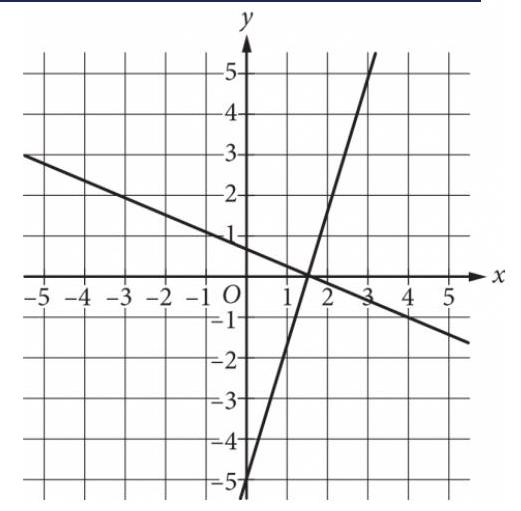
\includegraphics[max width=\textwidth, center]{2025_06_15_7d5ca6a095740ea44a32g-54}

Which of the following systems of equations has the same solution as the system of equations graphed above?\\
$y=0$\\
A. $x=\frac{3}{2}$\\
$y=\frac{3}{2}$\\
B. $x=0$\\
$y=0$\\
C. $x=1$\\
$y=1$\\
D. $x=0$

ID: 0d1dca87\\
$3 x+y=29$\\
$x=2$

If $(x, y)$ is the solution to the given system of equations, what is the value of $y$ ?

\section*{ID: 686b7cad}
A proposal for a new library was included on an election ballot. A radio show stated that 3 times as many people voted in favor of the proposal as people who voted against it. A social media post reported that 15,000 more people voted in favor of the proposal than voted against it. Based on these data, how many people voted against the proposal?\\
A. 7,500\\
B. 15,000\\
C. 22,500\\
D. 45,000

$$
\begin{gathered}
2 x+3 y=7 \\
10 x+15 y=35
\end{gathered}
$$

For each real number $r$, which of the following points lies on the graph of each equation in the $x y$-plane for the given system?\\
A. $\left(\frac{r}{5}+7,-\frac{r}{5}+35\right)$\\
B. $\left(-\frac{3 r}{2}+\frac{7}{2}, r\right)$\\
C. $\left(r, \frac{2 r}{3}+\frac{7}{3}\right)$\\
D. $\left(r,-\frac{3 r}{2}+\frac{7}{2}\right)$

\section*{ID: 5e08a055}
$$
y=6 x+18
$$

One of the equations in a system of two linear equations is given. The system has no solution. Which equation could be the second equation in the system?\\
A. $-6 x+y=18$\\
B. $-6 x+y=22$\\
C. $-12 x+y=36$\\
D. $-12 x+y=18$

\section*{ID: 0df106df}
An online bookstore sells novels and magazines. Each novel sells for \$4, and each magazine sells for \$1. If Sadie purchased a total of 11 novels and magazines that have a combined selling price of $\$ 20$, how many novels did she purchase?\\
A. 2\\
B. 3\\
C. 4\\
D. 5

ID: b544a348

$$
\begin{array}{r}
5 x+3 y=38 \\
x+3 y=10
\end{array}
$$

In the solution $(x, y)$ to the system of equations\\
above, what is the value of $x$ ?

\section*{ID: 7d89376f}
A discount airline sells a certain number of tickets, $x$, for a flight for $\$ 90$ each. It sells the number of remaining tickets, $y$, for $\$ 250$ each. For a particular flight, the airline sold 120 tickets and collected a total of $\$ 27,600$ from the sale of those tickets. Which system of equations represents this relationship between $x$ and $y$ ?\\
A. $\left\{\begin{array}{l}x+y=120 \\ 90 x+250 y=27,600\end{array}\right.$\\
, $x+y=120$\\
B. ${ }^{1} 90 x+250 y=120(27,600)$\\
$x+y=27,600$\\
C. ${ }^{1} 90 x+250 y=120(27,600)$\\
D. $\left\{\begin{array}{l}90 x=250 y \\ 120 x+120 y=27,600\end{array}\right.$

A movie theater charges $\$ 11$ for each full-price ticket and $\$ 8.25$ for each reducedprice ticket. For one movie showing, the theater sold a total of 214 full-price and reduced-price tickets for $\$ 2,145$. Which of the following systems of equations could be used to determine the number of full-price tickets, $f$, and the number of reduced-price tickets, $r$, sold?

A $f$ $f+r=2,145$\\
A. $11 f+8.25 r=214$ $f+r=214$\\
B. $11 f+8.25 r=2,145$ $f+r=214$\\
C. $8.25 f+11 r=2,145$\\
D. $f+r=2,145$\\
D. $8.25 f+11 r=214$

$$
\begin{gathered}
x+3 y=29 \\
3 y=11
\end{gathered}
$$

The solution to the given system of equations is $(x, y)$. What is the value of $x$ ?

\section*{ID: 44d65912}
Angela is playing a video game. In this game, players can score points only by collecting coins and stars. Each coin is worth $c$ points, and each star is worth $s$ points.

\begin{itemize}
  \item The first time she played, Angela scored 700 points. She collected 20 coins and 10 stars.
  \item The second time she played, Angela scored 850 points. She collected 25 coins and 12 stars.
\end{itemize}

Which system of equations can be used to correctly determine the values of $c$ and $s$ ?\\
A.

$$
\begin{aligned}
& 10 c+20 s=700 \\
& 12 c+25 s=850
\end{aligned}
$$

B.

$$
\begin{aligned}
& 20 c+10 s=700 \\
& 25 c+12 s=850
\end{aligned}
$$

C.

$$
\begin{aligned}
& 20 c+700 s=10 \\
& 25 c+850 s=12
\end{aligned}
$$

D.

$$
\begin{aligned}
& 700 c+20 s=10 \\
& 850 c+25 s=12
\end{aligned}
$$

\begin{center}
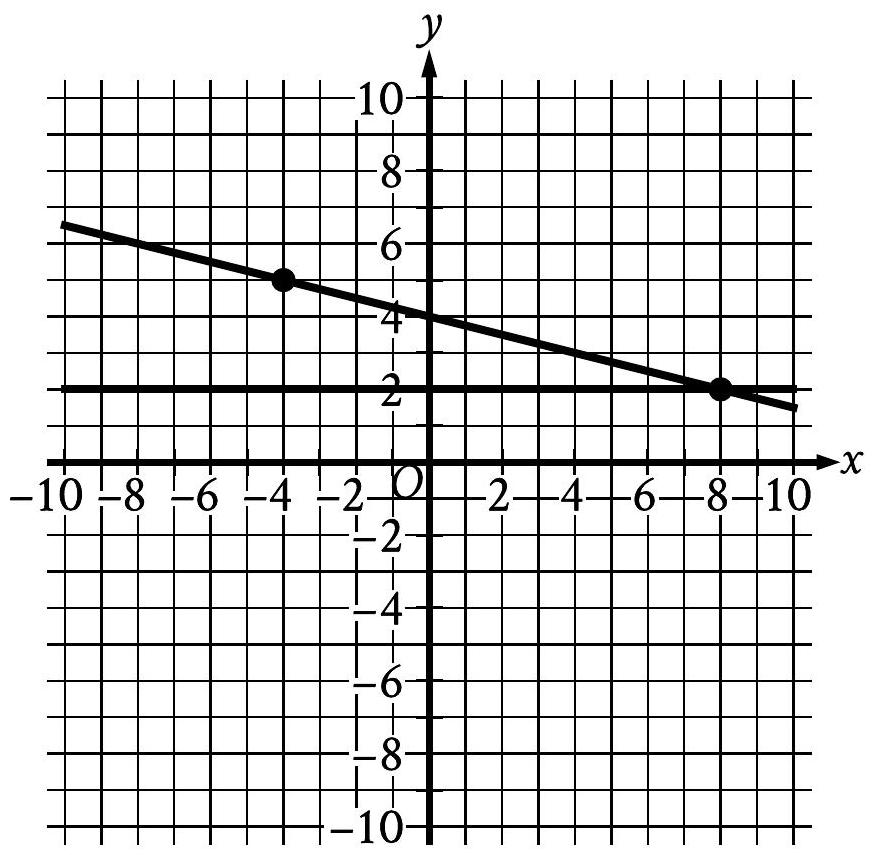
\includegraphics[max width=\textwidth]{2025_06_15_7d5ca6a095740ea44a32g-65}
\end{center}

If a new graph of three linear equations is created using the system of equations shown and the equation $x+4 y=-16$, how many solutions $(x, y)$ will the resulting system of three equations have?\\
A. Zero\\
B. Exactly one\\
C. Exactly two\\
D. Infinitely many

\section*{ID: 4b76c7f1}
$$
\begin{array}{r}
2 x+7 y=9 \\
8 x+28 y=a
\end{array}
$$

In the given system of equations, $a$ is a constant. If the system has infinitely many solutions, what is the value of $a$ ?\\
A. 4\\
B. 9\\
C. 36\\
D. 54


